\chapter[Aims]%
{Aims}

\begin{figure}[ht]
	\begin{center}
		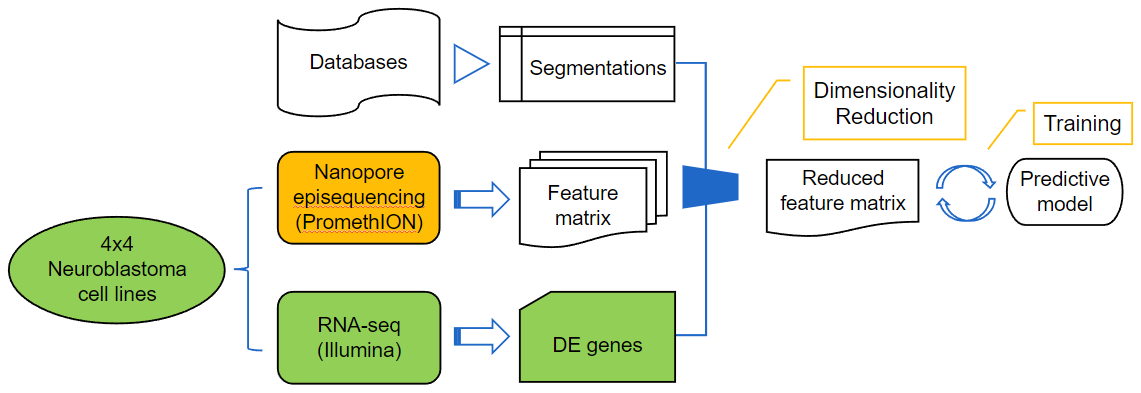
\includegraphics[width = \textwidth]{Fig/overview_temp.png}
	\end{center}
	\caption{Overview workflow.}
\end{figure}

The aim of this project is, first and foremost, to develop a machine learning model capable of accurately predicting ferroptosis sensitivity for a given tumor sample. To achieve the best possible performance, we will have to compare and determine the best feature reduction and modelling methodologies. 

In doing this, emphasis will be put on working annotation-agnostic whenever possible, te reduce reliance on prior knowledge and enhance confidence in the information extracted from the samples themselves. In light of these considerations, we will attempt multiple feature reduction strategies, and compare them as alternatives. Modelling performance will also be benchmarked for the various algorithms on offer. 

In post-analysis, we will reverse engineer the extracted features back to annotation, in hopes of discovering novel ferroptosis biomarkers. Finally, we will execute a comparative study of the methylation patterns between drug-sensitized tumors and wild type, non-sensitized cells from the same cell line.